\section{TWMM Description}
\subsection{Overview}
Unlike traditional CF-AMMs, the TWMM reframes IL and LVR as asset management challenges, akin to active trading strategies.

The TWMM system integrates a weighted portfolio strategy with an on-chain liquidity pool. It facilitates the exchange of underlying assets using oracle-provided prices. These oracles are designed to be LVR-aware, with their efficiency directly influenced by price volatility and the speed of their technical implementation. A key distinction from CF-AMMs is that TWMM orders, whose prices are determined by oracles, do not incur a price impact correlated with order quantity, thereby mitigating the significant price impact observed in large trades on CF-AMMs.

TWMM introduces the concept of assets possessing \textbf{target shares ($S_t$)}, which are denominated in a quote asset's value. In an ideal scenario, the share of each asset within the pool would perpetually fluctuate around a predefined target. These shares continuously deviate from their targets due to two primary factors: collateral rebalancing initiated by liquidity usage (trades) or fluctuations in the market prices of the assets themselves. The mechanism that enables this share rebalancing is an innovative fee model, which incentivizes the real-time share of each asset to converge towards its predetermined target or "ethalon" value.

 \subsection{Fees}
 The fee model is centered on a deviation metric that quantifies the difference between an asset's real-time share and its target share. As previously discussed, the \textbf{current share} ($S_c$) of an asset can diverge from its target share due to market price fluctuations and trading activity. The current share is calculated by dividing the asset's total value by the pool's Total Value Locked (\textbf{TVL}):
 
 \begin{equation}
 	\label{eq:current_share}
 	S_c = \frac{R \cdot P}{ Q_{lp} \cdot P_{lp}}
 \end{equation}
 
 In this equation, the numerator $R \cdot P$ is the asset's total value (reserves multiplied by price). The denominator, $R_{lp} \cdot P_{lp}$, represents the TVL of the pool, which is calculated by multiplying the total supply of LP tokens (their reserve $R_{lp}$) by the price of the LP token ($P_{lp}$).

\subsection{Deviation: The Core Metric}

\textbf{Deviation} is the fundamental metric that quantifies the difference between an asset's current share and its target share. For a specific asset , its \textbf{deviation value} ($D$) indicates the degree to which the asset is imbalanced relative to its target value within the TWMM pool. It is calculated as:

\begin{equation}
	\label{eq:deviation}
	D = S_{c} - S_{t}
\end{equation}

Here, $S_{c}$ and $S_{t}$ are the current and target shares for asset, respectively. A negative deviation value ($D < 0$) indicates a deficit of the asset in the pool, while a positive value ($D > 0$) signifies a surplus.

With $n$ representing the total number of assets, the deviation values adhere to two primary invariants:

\begin{equation}
	\label{eq:invariant_deviation}
	\sum_{i=1}^{n} D_i = 0, \qquad \sum_{i=1}^{n} |D_i| = 2 \cdot I
\end{equation}

The sum of all deviation values consistently equals zero. Concurrently, the sum of their absolute values defines the total imbalance of the pool, which is equal to twice the pool's aggregate imbalance rate ($I$).

This quantitative understanding of deviation is crucial for the TWMM's rebalancing mechanisms and fee model, which are elaborated upon in subsequent sections. The precise management of these deviations ensures the stability and efficiency of the system.

\subsection{Fee Structure}

Deviation plays a vital role in the fee structure of the TWMM. A fee is levied in the specific asset whose pool quantity is altered by an operation. These fees can be broken down into several components:

\begin{itemize}
	\item \textbf{Base Fee ($F_b$)}: A constant fee that is charged unconditionally on every operation.
	
	\item \textbf{Depeg Fee ($F_{dv}$)}: This dynamic fee serves the dual purpose of generating revenue and creating an economic incentive to maintain the pool's target allocations. It discourages operations that would increase an asset's imbalance by making them economically less appealing. The fee is a function of the asset's deviation before the operation ($D_o$) and after the operation ($D_n$). It is applied only when the absolute deviation of the asset increases as a result of the operation (i.e., $ \lvert D_n \rvert > \lvert D_o \rvert$). Conversely, if an operation causes the absolute deviation to decrease, this fee is waived.
	
	\item \textbf{Cashbacks ($F_{cb}$)}: Functioning as the inverse of the depeg fee, cashbacks are rebates that reward users for operations that reduce an asset's imbalance. A cashback is issued when a transaction moves an asset's current share closer to its target share (i.e., when $\lvert D_{new} \rvert < \lvert D_{old} \rvert$ and $\operatorname{sgn}(D_{old}) = \operatorname{sgn}(D_{new})$).
\end{itemize}

Synthesizing these individual components, the total effective fee ($F_{total}$) for any given operation is defined by the following general formula, which combines the base fee ($F_b$), the deviation fee ($F_{dv}$), and the cashback ($F_{cb}$):

\begin{equation}
	\label{eq:total_fee_formula}
	F_{total} = F_b + F_{dv} - F_{cb}
\end{equation}

The core concept is to calibrate fees based on the resulting change in an asset's deviation following a transaction. It is important to note that the \textbf{TWMM architecture supports various custom functions for calculating the deviation fee}, enabling flexible and adaptable fee structures. Examples of such functions include \textbf{linear} or \textbf{constant} models, in addition to more complex \textbf{curve-based} approaches.

\subsection{Fee Distribution}

Fees collected by the TWMM, excluding funds allocated for cashbacks, are distributed among three distinct parties, with configurable percentage shares for each:
\begin{itemize}
	\item LP token holders (liquidity providers)
	\item The pool owner or manager
	\item The protocol treasury
\end{itemize}

The distribution method varies by recipient. The share allocated to liquidity providers remains in the pool, increasing the quantity of the underlying assets and thereby causing the value of their LP tokens to appreciate.

Conversely, the shares designated for the pool owner and the protocol are distributed by minting new LP tokens. If the total quote value of the fees collected for the owner and protocol is $V_{col}$, the quantity of new LP tokens to be minted ($Q_{lpfee}$) is determined by the current LP token price ($P_{lp}$):

\begin{equation}
	\label{eq:fee_minting}
	Q_{lpfee} = \frac{V_{col}}{P_{lp}}
\end{equation}

This minting mechanism ensures that fee distributions to the owner and protocol do not directly withdraw assets from the pool. However, it is crucial to recognize that since fees are collected as assets within the pool, their collection inherently alters the pool's asset quantities. Consequently, the impact of both collected fees and awarded cashbacks must be accounted for when calculating the final deviation after a transaction.


\subsection{Deviation Limit}

The \textbf{deviation limit} is a control mechanism designed to restrict large-volume swaps that could cause a severe imbalance in the pool's asset composition.

An asset's deviation can exceed this specified limit passively as a result of market price fluctuations. When this occurs, transactions that reduce the asset's deviation are permitted to proceed normally, while any transaction that would further increase its absolute deviation is restricted.

Notably, a deviation fee may be waived even for trades that cause an asset's deviation to change sign (e.g., from a surplus to a deficit). The condition for this waiver is that the final absolute deviation must be less than the initial absolute deviation. Such transactions, even if large, are considered beneficial as they decrease the pool's overall imbalance and move the portfolio closer to its target equilibrium state $(I_{new} < I_{old})$ as described in deviation invariant \ref{eq:invariant_deviation}.

\subsection{Deviation Fee}
To model the deviation fee, we first define two auxiliary components: the initial deviation before a transaction and the change in deviation resulting from it.

First, the initial deviation ($D_{old}$) represents the asset's deviation state immediately before a swap. Consistent with Equation \ref{eq:deviation}, it is defined using the asset's reserve ($R$) in TWMM pool, its price ($P$), its target share ($S_t$), and the pool's Total Value Locked ($R_{lp} \cdot P_{lp}$):
\begin{equation}
	\label{eq:deviation_old_function_formula}
	D_{old} = S_t - \frac{R \cdot P}{R_{lp} \cdot P_{lp}}
\end{equation}	

Second, the change in deviation, $\Delta D$, is a function of the change in the asset's quantity, $\Delta Q$, resulting from the swap. It is calculated as:
\begin{equation}
	\label{eq:deviation_delta_function_formula}
	\Delta D(\Delta Q) = \frac{ \Delta Q \cdot P}{Q_{lp} \cdot P_{lp}}
\end{equation}	

The deviation fee, $F_{dv}$, is modeled as a piecewise linear function. It applies a fee only if a transaction increases the absolute deviation of the asset. The general form, parameterized by a multiplier $K$ and a constant $B$, is:
\begin{equation}
	\label{eq:basic_deviation_function}
	F_{dv}(\Delta D) = \begin{cases} 
		K \cdot \lvert D_{old} + \Delta D \rvert + B, & \text{if } \lvert D_{old} + \Delta D \rvert > \lvert D_{old} \rvert, \\
		0, & \text{otherwhise.}
	\end{cases}	
\end{equation}

The illustration of this function is:

\begin{figure}[h!]
	\centering
	\begin{subfigure}{0.4\textwidth}
		\centering
		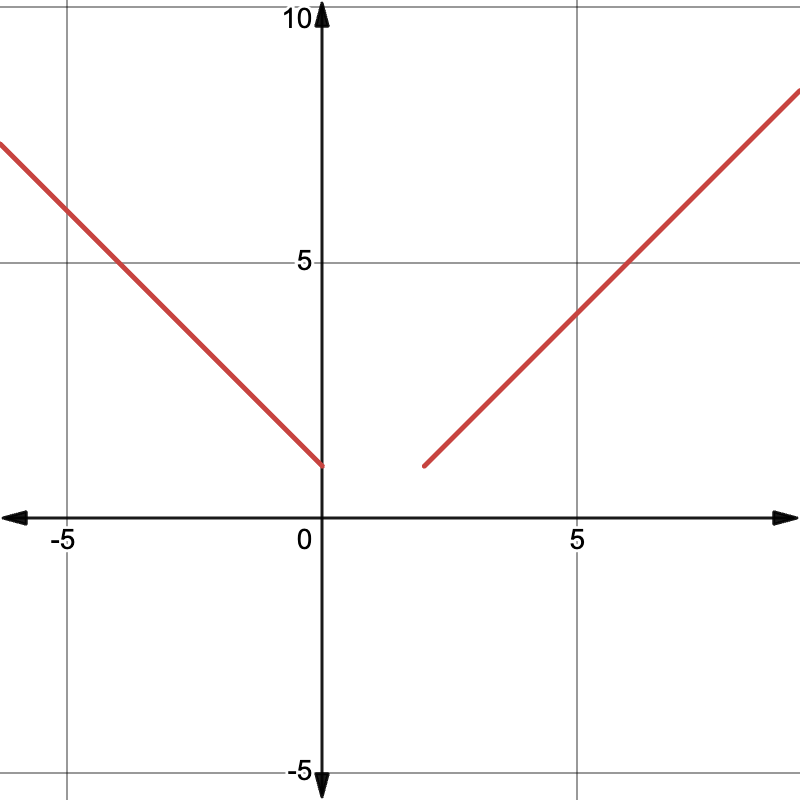
\includegraphics[width=\linewidth]{deviation_function_no_offset.png} 
		\caption{Deviation function with $B = 0$ }
		\label{fig:img1}
	\end{subfigure}
	\hfill 
	\begin{subfigure}{0.4\textwidth}
		\centering
		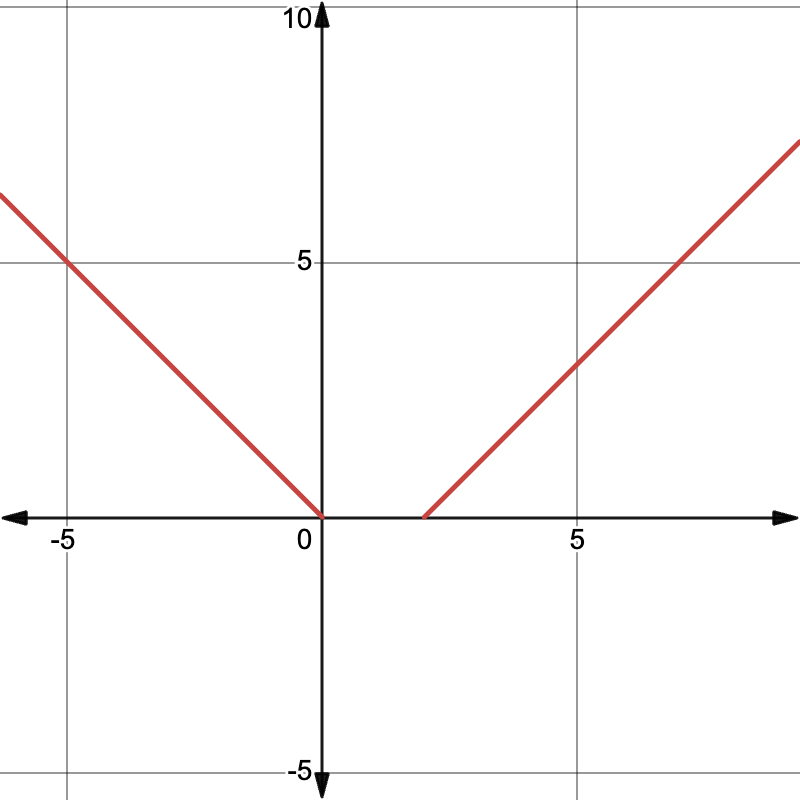
\includegraphics[width=\linewidth]{deviation_function_with_offset.png} 
		\caption{Deviation function with $B = - K \lvert D_{old} \rvert$ }
		\label{fig:img2}
	\end{subfigure}
    \caption{Linear deviation functions}
	\label{fig:img3}
\end{figure}
\FloatBarrier

To refine the fee model, we first adjust the linear function from Equation \ref{eq:basic_deviation_function}. The previous form results in a fee greater than $B$ as soon as the deviation increases. To ensure the fee is exactly $B$ at the threshold where deviation begins to increase, and grows proportionally to the \textit{increase} in absolute deviation, the function is recalibrated as follows:
\begin{equation}
	\label{eq:general_deviation_function}
	F_{dv}(\Delta D) = \begin{cases} 
		K \cdot (\lvert D_{old} + \Delta D \rvert - \lvert D_{old} \rvert) + B, & \text{if } \lvert D_{old} + \Delta D \rvert > \lvert D_{old} \rvert, \\
		0, & \text{otherwhise.} 
	\end{cases}	
\end{equation}

A further refinement is necessary to account for the recursive impact of the fee itself. The collected fee alters the final input or output amount, which in turn influences the deviation value used to calculate the fee. This self-referential dependency requires an implicitly defined function. We introduce a parameter, deviation fee to cashback ratio ($r_d$), which is related to the fee's allocation toward the cashback fund.

For an asset being added to the pool, the implicit fee function, $F_{dIn}$, which accounts for the portion of the fee retained by the pool, is:
\begin{equation}
	\label{eq:deviation_in_function}
	F_{dIn}(\Delta D_{in}) = K \cdot (\lvert D_{oIn} + \Delta D_{in} \cdot [1 - r_{d} \cdot F_{dIn}(\Delta D_{in}) ] \rvert - \lvert D_{oIn} \rvert) + B  
\end{equation}
Here, the gross change in deviation, $\Delta D_{in}$, is adjusted by a factor dependent on the final fee itself.

Similarly, for an asset being withdrawn from the pool (the "out" asset), a corresponding implicit function, $F_{dOut}$, is required to model the fee's effect on the final withdrawal amount:
% system with a proper equation of where it's applied?
% simplification here?
\begin{equation}
	\label{eq:deviation_out_function}
	F_{dOut}(\Delta D_{out}) = K \cdot (\lvert D_{oOut} + \Delta D_{out} \cdot [1 + r_{d} \cdot F_{dOut}(\Delta D_{out})] \rvert - \lvert D_{oOut} \rvert) + B 
\end{equation}

\subsection{Cashbacks}
\textbf{Cashbacks} are financial incentives provided to users who execute trades that shift an underlying asset's share within the \textbf{TWMM} closer to its designated target share.

The cashback mechanism is funded by the deviation fees collected from prior operations that increased the pool's imbalance. These accumulated funds are then distributed to users whose transactions reduce an asset's deviation. The magnitude of the distributed cashback is directly proportional to the extent of the deviation reduction. For instance, if a transaction reduces an asset's d 
The total accumulated fund available for cashback distribution for a given asset is denoted by $C$. The specific cashback amount, $F_{cb}$, is calculated using the absolute deviation before the operation, $|D_o|$, and after the operation, $|D_n|$, as described by the formula:

\begin{equation}
	\label{eq:cashback_formula}
	F_{cb} = \frac{(|D_o| - |D_n|) \cdot C}{|D_o| \cdot \Delta Q} 
\end{equation}

A key design consideration is that this calculation is non-recursive. While the awarded cashback could theoretically be redeposited and create a secondary impact on deviation, calculating this effect recursively is avoided as it could create unstable feedback loops that overdistribute and overincentivise trades. For this reason, the secondary impact is not considered. 

Furthermore, to ensure stability and efficient value distribution, the cashback award is capped by  maximum cashback ($C_{max}$) - a maximum ratio relative to the size of the user's input quantity, $\Delta Q$. General cashback function derived from \ref{eq:cashback_formula} looks like:

\begin{equation}
	\label{eq:invariant_swap_cashback_function}
	F_{\mathrm{cb}}(\Delta Q)
	=
	\begin{cases}
		\displaystyle
		\begin{aligned}
			\min\Bigl(
			\frac{\lvert D_{old}\rvert
				- \bigl\lvert D_{old}
				+ \Delta D\bigr\rvert}
			{\lvert D_{old}\rvert}
			\cdot \frac{C}{\Delta Q},C_{max}
			\Bigr),
		\end{aligned}
		&
		\begin{aligned}
			&\text{if }\lvert D_{old} + \Delta D\rvert
			< \lvert D_{old}\rvert\\
			& \text{and }\operatorname{sgn}(D_{old})
			= \operatorname{sgn}(D_{new}),
		\end{aligned}
		\\[3ex]
		0,
		& \text{otherwise.}
	\end{cases}
\end{equation}



The calculation of the cashback rate, denoted as $F_{cb}$, requires careful constraint to ensure it properly incentivizes balancing the pool without creating instabilities. The models differ slightly for assets being deposited versus assets being withdrawn.

\subsubsection*{Cashback for Input Asset (F\textsubscript{cIn})}

For an input asset ($\Delta Q_{in} > 0$) that is reducing a deficit ($D_{oIn} < 0$), the cashback must be constrained to prevent the final deviation from overshooting past zero.
To prevent the cashback from causing the final deviation to cross zero, we introduce a second constraint, $C_z$. This value represents the maximum cashback rate that results in a final deviation of exactly zero.
\begin{equation}
	\label{eq:cashback_constraint for_amount_in}
	D_{oIn} + \Delta D_{in} \cdot (1 + C_z) = 0 \iff C_z = -\left(\frac{D_{oIn}}{\Delta D_{in}} + 1\right)
\end{equation}

\begin{equation}
	\label{eq:invariant_swap_cashback_in_function}
	F_{cIn}(\Delta Q_{in}) = \min\left(\frac{\lvert D_{oIn} \rvert - \lvert D_{oIn} + \Delta D_{in} \rvert}{ \lvert D_{oIn} \rvert} \cdot \frac{C_{in}}{\Delta Q_{in}}, C_{max}, C_z\right)
\end{equation}

Under the specific condition that the transaction reduces the deficit but does not eliminate it (i.e., $D_{oIn} + \Delta D_{in} < 0$), the formula can be simplified:
\begin{equation}
	\label{eq:invariant_swap_cashback_in_function_simplified}
	F_{cIn}(\Delta Q_{in}) = \min\left(-\frac{ \Delta D_{in}}{ D_{oIn}} \cdot \frac{C_{in}}{\Delta Q_{in}}, C_{max}, C_z\right)
\end{equation}


Combining these constraints yields the final piecewise function for the input asset cashback rate. The rate is the minimum of the calculated proportional rate, the global maximum rate ($C_{max}$), and the zero-crossing rate ($C_z$). A cashback is only awarded if the transaction does not push the deviation into a surplus.
\begin{equation}
	\label{eq:swap_invariant_cashback_in_function_final}
	F_{cIn}(\Delta Q_{in}) = \begin{cases}
		\begin{aligned} \min\left(-\frac{ \Delta D_{in}}{ D_{oIn}} \cdot \frac{C_{in}}{\Delta Q_{in}}, C_{max}, -\left(\frac{D_{oIn}}{\Delta D_{in}} + 1\right)\right) \end{aligned}, & \text{if } D_{oIn} + \Delta D_{in} < 0, \\
		0, & \text{otherwhise.}
	\end{cases}	
\end{equation}

\subsubsection*{Cashback for Output Asset (F\textsubscript{cOut})}
The logic for an output asset that reduces a surplus ($D_{oOut} > 0$) is symmetrical. The cashback is drawn from the collected reserve $C_{out}$ and does not create secondary deviation effects. The general and simplified formulas are analogous to the input asset case:
\begin{equation}
	\label{eq:invariant_swap_cashback_out_function}
	F_{cOut}(\Delta Q_{out}) = \min\left(\frac{\lvert D_{oOut} \rvert - \lvert D_{oOut} - \Delta D_{out} \rvert}{ \lvert D_{oOut} \rvert} \cdot \frac{C_{out}}{|\Delta Q_{out}|}, C_{max}\right)
\end{equation}

Assuming the transaction reduces but does not eliminate the surplus ($D_{oOut} - \Delta D_{out} > 0$), this simplifies to:
\begin{equation}
	\label{eq:invariant_swap_cashback_out_function_simplified}
	F_{cOut}(\Delta Q_{out}) = \min\left(\frac{ \Delta D_{out}}{ D_{oOut}} \cdot \frac{C_{out}}{|\Delta Q_{out}|}, C_{max}\right)
\end{equation}

The final function for the output asset cashback rate is therefore given as:
\begin{equation}
	\label{eq:swap_invariant_cashback_out_function_final}
	F_{cOut}(\Delta Q_{out}) = \begin{cases}
		\begin{aligned} \min\left(\frac{ \Delta D_{out}}{ D_{oOut}} \cdot \frac{C_{out}}{|\Delta Q_{out}|}, C_{max}\right) \end{aligned}, & \text{if } D_{oOut} - \Delta D_{out} > 0, \\
		0, & \text{otherwhise.}
	\end{cases}	
\end{equation}

\subsection{Full TWMM swap invariant}
The swap invariant defines the fundamental relationship between the amount of an asset deposited into the pool ($\Delta Q_{in}$) and the amount of another asset withdrawn ($\Delta Q_{out}$). This relationship incorporates the asset prices ($P_{in}, P_{out}$), the respective base fees ($F_{bIn}, F_{bOut}$), and the net directional fees ($F_{in}, F_{out}$), which represent the combined effect of deviation fees and cashbacks. The invariant is expressed as:

\begin{equation}
	\label{eq:swap_invariant}
	\Delta Q_{in} \cdot P_{in} \cdot (1 - F_{bIn} - F_{in}(\Delta Q_{in})) = \Delta Q_{out} \cdot P_{out} \cdot (1 + F_{bOut} + F_{out}(\Delta Q_{out}))
\end{equation}

Because the base fee ($F_{base}$) is retained in the form of the asset being transacted and thus affects the pool's deviation, its collection can be split between the input and output assets. We define these user-configurable portions as $F_{bIn}$ and $F_{bOut}$, which must adhere to the constraint:
\begin{equation}
	F_{base} = F_{bIn} + F_{bOut}
\end{equation}

The net directional fee terms, $F_{in}$ and $F_{out}$, are composite values. They are derived by combining the previously defined deviation fee functions (e.g., Equation \ref{eq:deviation_in_function}) and cashback functions (e.g., Equation \ref{eq:swap_invariant_cashback_in_function_final}). Merging these components yields the final, comprehensive fee function used in the swap invariant for the input asset:

\begin{equation}
	\label{eq:fee_in_formula}
	F_{\mathrm{in}}(\Delta Q_{\mathrm{in}})
	=
	\begin{cases}
		-\displaystyle
		\min\Bigl(
		\frac{\Delta D_{\mathrm{in}}}{D_{o\mathrm{In}}}
		\cdot \frac{C_{\mathrm{in}}}{\Delta Q_{\mathrm{in}}},
		\;C_{m},
		\;-\Bigl(\frac{D_{o\mathrm{In}}}{\Delta D_{\mathrm{in}}} + 1\Bigr)
		\Bigr),
		& \text{if } D_{o\mathrm{In}} + \Delta D_{\mathrm{in}} < 0,
		\\[2ex]

		\displaystyle
		\begin{aligned}
			K\Bigl(&\bigl\lvert\,D_{o\mathrm{In}}
			+ \Delta D_{\mathrm{in}}
			\bigl[1 - r_{d}\,F_{ \mathrm{In} }(\Delta D_{\mathrm{in}})\bigr]
			\bigr\rvert \\
			&\quad - \lvert D_{o\mathrm{In}}\rvert\Bigr)
			+ B,
		\end{aligned}
		& \text{if } D_{o\mathrm{In}} + \Delta D_{\mathrm{in}}
		> \lvert D_{o\mathrm{In}}\rvert,
		\\[2ex]
		0,
		& \text{otherwhise.}
	\end{cases}
\end{equation}


Following the same procedure, the net directional fee for the output asset, $F_{out}$, is derived by combining the cashback and deviation fee functions applicable to asset withdrawals:

\begin{equation}
	\label{eq:fee_out_formula}
	F_{\mathrm{out}}(\Delta Q_{\mathrm{out}})
	=
	\begin{cases}
		-\displaystyle\min\Bigl(
		\frac{\Delta D_{\mathrm{out}}}{D_{o\mathrm{Out}}}
		\cdot \frac{C_{\mathrm{out}}}{\Delta Q_{\mathrm{out}}},
		\;C_{\max}
		\Bigr),
		& \text{if } D_{o\mathrm{Out}} - \Delta D_{\mathrm{out}} > 0,
		\\[2ex]
		\displaystyle
		\begin{aligned}
			\Bigl(&\bigl\lvert\,D_{o\mathrm{Out}}
			+ \Delta D_{\mathrm{out}}
			\bigl[1 + r_{d}\,F_{d\mathrm{Out}}(\Delta D_{\mathrm{out}})\bigr]
			\bigr\rvert \\
			&\quad - \lvert D_{o\mathrm{Out}}\rvert\Bigr) \cdot K
			+ B,
		\end{aligned}
		& \text{if } D_{o\mathrm{Out}}
		-\Delta D_{\mathrm{out}}
		< -\lvert D_{o\mathrm{Out}}\rvert,
		\\[2ex]
		0,
		& \text{otherwise.}
	\end{cases}
\end{equation}

To execute a swap, a user must identify a pair of quantities, $(\Delta Q_{in}, \Delta Q_{out})$, that satisfies the swap invariant defined in Equation \ref{eq:swap_invariant}. In practice, finding the optimal trade that maximizes the output value for a given input may require iteratively solving this equation, a process that must account for potential fluctuations in market prices during transaction construction.

\subsection{Liquidity Provision and Removal}

Liquidity provision and removal are the operations for depositing assets into the pool to mint LP tokens, or burning LP tokens to withdraw underlying assets. Unlike swaps which exchange one pool asset for another, these operations always involve a transaction between one or more pool assets and the pool's own LP tokens. This allows to apply less deviation impact for big amount of liqudiity provision or removal

Because these operations alter the total supply of LP tokens ($Q_{lp}$), the denominator of the share calculation (i.e., the Total Value Locked) changes during the transaction itself. This requires a redefinition of our deviation formulas (the deviation old formula (\ref{eq:deviation_old_function_formula}) and deviation delta formula (\ref{eq:deviation_delta_function_formula})). For a liquidity operation involving a quantity $\Delta Q$ of a single asset and $\Delta Q_{lp}$ of LP tokens, we define the initial deviation and the change in deviation as follows:

\begin{equation}
	\label{eq:old_deviation_function_formula_for_lp}
	D_{old}(\Delta Q, \Delta Q_{lp}) = S_t - \frac{R \cdot P}{R_{lp} \cdot P_{lp}}
\end{equation}	

\begin{equation}
	\label{eq:deviation_delta_function_formula_for_lp}
	\Delta D(\Delta Q, \Delta Q_{lp}) = \frac{\Delta Q \cdot P}{\Delta Q_{lp} \cdot P_{lp}} 
\end{equation}	

It is important to note that the LP token itself is not subject to deviation fees or cashbacks. As a derivative representing a share of the entire pool, it is not considered a constituent asset with a target share.

\subsection{Multi-Asset Liquidity Invariant}
While liquidity can be provided with a single asset, this action inherently unbalances the pool's composition, leading to a significant deviation impact and potentially high fees for the liquidity provider. To mitigate this, the TWMM is designed to support multi-asset liquidity provision and removal. By depositing or withdrawing assets in proportions that align with the pool's target shares, users can add or remove liquidity with minimal deviation impact and associated costs.

The relationship between the assets being transacted and the LP tokens is governed by the following invariants. For minting LP tokens by depositing $n$ assets, the invariant is:
\begin{equation}
	\label{eq:invariant_lp_mint}
	\sum_{i=1}^{n} 
	(1 -  F_{base} - F_{in}(\Delta Q_{in}, \Delta Q_{lp})) \Delta Q_{in} P_{in}  
	= 
	\Delta Q_{lp} P_{lp} 
\end{equation}
This equation states that the value of the minted LP tokens equals the sum of the net values of all deposited assets after their respective fees are deducted.

Symmetrically, the invariant for burning LP tokens to withdraw $n$ assets is:
\begin{equation}
	\label{eq:invariant_lp_mint}
	\Delta Q_{lp} P_{lp}  =
	\sum_{o=1}^{n} 
	(1 + F_{base} + F_{out}(\Delta Q_{out}, \Delta Q_{lp})) \Delta Q_{out} P_{out}  
\end{equation}

These liquidity operations can be integrated into a generalized invariant that holistically describes all possible interactions with the pool.